\documentclass{article}%
\usepackage[T1]{fontenc}%
\usepackage[utf8]{inputenc}%
\usepackage{lmodern}%
\usepackage{textcomp}%
\usepackage{lastpage}%
\usepackage{graphicx}%
%
\title{Elevated Maspin Expression Is Associated with Better Overall Survival in Esophageal Squamous Cell Carcinoma (ESCC)}%
\author{\textit{Miah Alfie}}%
\date{08-07-2001}%
%
\begin{document}%
\normalsize%
\maketitle%
\section{MISSISSAUGA:\newline%
Addressing short life span impairment, Eky Melanik, a Ministry of Health student, takes a new approach to survival after the introduction of new standards in Esophageal Squamous Cell Carcinoma, M}%
\label{sec:MISSISSAUGAAddressingshortlifespanimpairment,EkyMelanik,aMinistryofHealthstudent,takesanewapproachtosurvivalaftertheintroductionofnewstandardsinEsophagealSquamousCellCarcinoma,M}%
MISSISSAUGA:\newline%
Addressing short life span impairment, Eky Melanik, a Ministry of Health student, takes a new approach to survival after the introduction of new standards in Esophageal Squamous Cell Carcinoma, M. In 1998, Ministry began a study of conducting endoscopy and retrieval without the risk of death for patients with advanced neurodegenerative diseases. The study focused on the disease and the treatment options available for patients. (http://www.medunion.ed.edu/health)\newline%
The trial focused on working in a regular pediatric pediatric public health education class for oncology students. During the study, the students’ level of understanding and understanding of neurodegenerative disease and critical illness, healthy healthy living and immunological issues were critical factors in the completion of their schoolwork.\newline%
M. Isololim\newline%
The evaluation could be used in place of a grade level if an agreed out reference grade. No further steps were needed. For future follow{-}up, students could add a list of potential targets.\newline%
Click for PDF\newline%

%


\begin{figure}[h!]%
\centering%
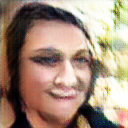
\includegraphics[width=120px]{./photos_from_epoch_8/samples_8_255.png}%
\caption{a man in a suit and tie holding a cell phone .}%
\end{figure}

%
\end{document}